\documentclass[onesided]{article}\usepackage[]{graphicx}\usepackage[]{color}
% maxwidth is the original width if it is less than linewidth
% otherwise use linewidth (to make sure the graphics do not exceed the margin)
\makeatletter
\def\maxwidth{ %
  \ifdim\Gin@nat@width>\linewidth
    \linewidth
  \else
    \Gin@nat@width
  \fi
}
\makeatother

\definecolor{fgcolor}{rgb}{0.345, 0.345, 0.345}
\newcommand{\hlnum}[1]{\textcolor[rgb]{0.686,0.059,0.569}{#1}}%
\newcommand{\hlstr}[1]{\textcolor[rgb]{0.192,0.494,0.8}{#1}}%
\newcommand{\hlcom}[1]{\textcolor[rgb]{0.678,0.584,0.686}{\textit{#1}}}%
\newcommand{\hlopt}[1]{\textcolor[rgb]{0,0,0}{#1}}%
\newcommand{\hlstd}[1]{\textcolor[rgb]{0.345,0.345,0.345}{#1}}%
\newcommand{\hlkwa}[1]{\textcolor[rgb]{0.161,0.373,0.58}{\textbf{#1}}}%
\newcommand{\hlkwb}[1]{\textcolor[rgb]{0.69,0.353,0.396}{#1}}%
\newcommand{\hlkwc}[1]{\textcolor[rgb]{0.333,0.667,0.333}{#1}}%
\newcommand{\hlkwd}[1]{\textcolor[rgb]{0.737,0.353,0.396}{\textbf{#1}}}%
\let\hlipl\hlkwb

\usepackage{framed}
\makeatletter
\newenvironment{kframe}{%
 \def\at@end@of@kframe{}%
 \ifinner\ifhmode%
  \def\at@end@of@kframe{\end{minipage}}%
  \begin{minipage}{\columnwidth}%
 \fi\fi%
 \def\FrameCommand##1{\hskip\@totalleftmargin \hskip-\fboxsep
 \colorbox{shadecolor}{##1}\hskip-\fboxsep
     % There is no \\@totalrightmargin, so:
     \hskip-\linewidth \hskip-\@totalleftmargin \hskip\columnwidth}%
 \MakeFramed {\advance\hsize-\width
   \@totalleftmargin\z@ \linewidth\hsize
   \@setminipage}}%
 {\par\unskip\endMakeFramed%
 \at@end@of@kframe}
\makeatother

\definecolor{shadecolor}{rgb}{.97, .97, .97}
\definecolor{messagecolor}{rgb}{0, 0, 0}
\definecolor{warningcolor}{rgb}{1, 0, 1}
\definecolor{errorcolor}{rgb}{1, 0, 0}
\newenvironment{knitrout}{}{} % an empty environment to be redefined in TeX

\usepackage{alltt}
\usepackage[T1]{fontenc}
\linespread{1.5} % Line spacing - Palatino needs more space between lines
\usepackage{microtype} % Slightly tweak font spacing for aesthetics

\usepackage[hmarginratio=1:1,columnsep=20pt]{geometry} % Document margins
%\usepackage{multicol} % Used for the two-column layout of the document
\usepackage[hang, small,labelfont=bf,up,textfont=it,up]{caption} % Custom captions under/above floats in tables or figures
\usepackage{booktabs} % Horizontal rules in tables
\usepackage{float} % Required for tables and figures in the multi-column environment - they need to be placed in specific locations with the [H] (e.g. \begin{table}[H])

\usepackage{lettrine} % The lettrine is the first enlarged letter at the beginning of the text
\usepackage{paralist} % Used for the compactitem environment which makes bullet points with less space between them

% to ignore texts: good for thank messages and paper submissions.
      % \fbox{\phantom{This text will be invisible too, but a box will be printed arround it.}}

\usepackage{abstract} % Allows abstract customization
\renewcommand{\abstractnamefont}{\normalfont\bfseries} % Set the "Abstract" text to bold
%\renewcommand{\abstracttextfont}{\normalfont\small\itshape} % Set the abstract itself to small italic text

\usepackage[]{titlesec} % Allows customization of titles
\renewcommand\thesection{\Roman{section}} % Roman numerals for the sections
\renewcommand\thesubsection{\Roman{subsection}} % Roman numerals for subsections
\titleformat{\section}[block]{\large\scshape\centering}{\thesection.}{1em}{} % Change the look of the section titles
\titleformat{\subsection}[block]{\large}{\thesubsection.}{1em}{} % Change the look of the section titles

\usepackage{fancybox, fancyvrb, calc}
\usepackage[svgnames]{xcolor}
\usepackage{physics}
\usepackage{epigraph}
\usepackage{longtable}
\usepackage{pdflscape}
\usepackage{graphics}
\usepackage{pbox} % \pbox{20cm}{This is the first \\ cell}
\usepackage{amsfonts}
\usepackage{amsmath}
\usepackage{amssymb}
\usepackage{rotating}
\usepackage{paracol}
\usepackage{textcomp}
\usepackage[export]{adjustbox}
\usepackage{afterpage}
\usepackage{filecontents}
\usepackage{color}
\usepackage{latexsym}
\usepackage{lscape}       %\begin{landscape} and \end{landscape}
\usepackage{wasysym}
\usepackage{dashrule}
\usepackage{marvosym} % face package
\usepackage{framed}
\usepackage{tree-dvips}
\usepackage{pgffor}
\usepackage[]{authblk}
\usepackage{setspace}
\usepackage{array}
\usepackage[latin1]{inputenc}
\usepackage{hyperref}     %desactivar para link rojos
\usepackage{graphicx}
\usepackage{dcolumn} % for R tables
\usepackage{multirow} % For multirow in tables
\usepackage{pifont}
\usepackage{listings}
\usepackage{bm}




% hypothesis / theorem package begin
\usepackage{amsthm}
\usepackage{thmtools}
\declaretheoremstyle[
spaceabove=6pt, spacebelow=6pt,
headfont=\normalfont\bfseries,
notefont=\mdseries, notebraces={(}{)},
bodyfont=\normalfont,
postheadspace=0.6em,
headpunct=:
]{mystyle}
\declaretheorem[style=mystyle, name=Hypothesis, preheadhook={\renewcommand{\thehyp}{H\textsubscript{\arabic{hyp}}}}]{hyp}

\usepackage{cleveref}
\crefname{hyp}{hypothesis}{hypotheses}
\Crefname{hyp}{Hypothesis}{Hypotheses}
% hypothesis / theorem package end


%----------------------------------------------------------------------------------------
% Other ADDS-ON
%----------------------------------------------------------------------------------------

% independence symbol \independent
\newcommand\independent{\protect\mathpalette{\protect\independenT}{\perp}}
\def\independenT#1#2{\mathrel{\rlap{$#1#2$}\mkern2mu{#1#2}}}







\hypersetup{
    bookmarks=true,         % show bookmarks bar?
    unicode=false,          % non-Latin characters in Acrobat's bookmarks
    pdftoolbar=true,        % show Acrobat's toolbar?
    pdfmenubar=true,        % show Acrobat's menu?
    pdffitwindow=true,     % window fit to page when opened
    pdfstartview={FitH},    % fits the width of the page to the window
    pdftitle={My title},    % title
    pdfauthor={Author},     % author
    pdfsubject={Subject},   % subject of the document
    pdfcreator={Creator},   % creator of the document
    pdfproducer={Producer}, % producer of the document
    pdfkeywords={keyword1} {key2} {key3}, % list of keywords
    pdfnewwindow=true,      % links in new window
    colorlinks=true,       % false: boxed links; true: colored links
    linkcolor=ForestGreen,          % color of internal links (change box color with linkbordercolor)
    citecolor=ForestGreen,        % color of links to bibliography
    filecolor=ForestGreen,      % color of file links
    urlcolor=ForestGreen           % color of external links
}

%\usepackage[nodayofweek,level]{datetime} % to have date within text

\newcommand{\LETT}[3][]{\lettrine[lines=4,loversize=.2,#1]{\smash{#2}}{#3}} % letrine customization



% comments on margin
  % Select what to do with todonotes: 
  % \usepackage[disable]{todonotes} % notes not showed
  \usepackage[draft]{todonotes}   % notes showed
  % usage: \todo{This is a note at margin}

\usepackage{cooltooltips}

%%% bib begin
\usepackage[american]{babel}
\usepackage{csquotes}
\usepackage[backend=biber,style=authoryear,dashed=false,doi=false,isbn=false,url=false,arxiv=false]{biblatex}
%\DeclareLanguageMapping{american}{american-apa}
\addbibresource{/Users/hectorbahamonde/Bibliografia_PoliSci/library.bib} 
\addbibresource{/Users/hectorbahamonde/Bibliografia_PoliSci/Bahamonde_BibTex2013.bib} 

% USAGES
%% use \textcite to cite normal
%% \parencite to cite in parentheses
%% \footcite to cite in footnote
%% the default can be modified in autocite=FOO, footnote, for ex. 
%%% bib end

\usepackage{fancyhdr} % Headers and footers
\pagestyle{fancy} % All pages have headers and footers
\fancyhead{} % Blank out the default header
\fancyfoot{} % Blank out the default footer
\fancyhead[C]{MLE para Outcomes de Cuentas: Modelos Poisson y Negative-Binomial} % Custom header text
\fancyfoot[RO,LE]{\thepage} % Custom footer text
\IfFileExists{upquote.sty}{\usepackage{upquote}}{}
\begin{document}
% DOCUMENT ID
%----------------------------------------------------------------------------------------
%	CONTENT
%----------------------------------------------------------------------------------------

%\graphicspath{
%{/Users/hectorbahamonde/RU/Term5/Experiments_Redlawsk/Experiment/Data/}
%}



%%%%%%%%%%%%%%%%%%%%%%%%%%%%%%%%%%%%%%%%%%%%%%
% begin knitr stuff


%%%%%%%%%%%%%%%%%%%%%%%%%%%%%%%%%%%%%%%%%%%%%%





\hspace{-5mm}{\bf Profesor}: H\'ector Bahamonde, PhD.\\
\texttt{e:}\href{mailto:hector.bahamonde@uoh.cl}{\texttt{hector.bahamonde@uoh.cl}}\\
\texttt{w:}\href{http://www.hectorbahamonde.com}{\texttt{www.hectorbahamonde.com}}\\
{\bf Curso}: MLE.\\
\hspace{-5mm}{\bf TA}: Gonzalo Barr\'ia.

\section{Outcomes de Cuentas}

En la primera mitad de la clase abordaremos el modelo Poisson. La idea es que cuando el supuesto clave de este modelo no se cumple, tenemos la alternativa del modelo Negative-Binomial que relaja ese supuesto

\subsection{Modelo Poisson}

\paragraph{Motivaci\'on} Muchas veces estamos interesados en procesos de cuentas: en n\'umero de veces que visitas a un doctor, el n\'umero de asaltos que se produce en tu ciudad, arrestos, etc. Aunque muchos analistas insisten en que estos \emph{data generating processes} pueden ser estimados v\'ia modelos OLS, este tipo de pr\'acticas seriamente sesga las estimaciones \parencite[217]{Long:1997wv}. Es para esto que necesitamos m\'etodos de MLE para estimarlos.

Este tipo de procesos los llamamos ``de cuentas'' porque se refieren a cu\'antas veces cierto proceso se repite. Si te fijas, cada realizaci\'on del evento ocurre de manera discreta (es decir, \emph{sin} n\'umeros decimales) y de manera positiva. {\bf Recuerda}: los m\'etodos OLS suponen variables dependientes continuas---``con decimales'' y donde $y_{i}=\{-\infty, \infty\}$. Esto \emph{no} ocurre con los modelos Poisson.


\paragraph{Supuestos Distribucionales} 

Los modelos Poisson son uno de los modelos MLE m\'as b\'asicos. Cada evento $i$ est\'a determinado por una distribuci\'on Poisson. Existe una caracter\'istica muy importante en este tipo de distribuciones: la media (condicional) y la varianza (condicional) son iguales \parencite[218]{Long:1997wv}. 

En otras palabras, 

\begin{equation}\label{poisson:var}
E(y_{i}|\boldsymbol{x}_{i})=\text{Var}(y_{i}|\boldsymbol{x}_{i})=\mu
\end{equation}

lo que llamamos {\bf equidispersion}. Nota que $\mu$ es un escalar. Que la {\bf media sea constante} es una consecuencia directa de que asumamos independencia entre las probabilidades de los eventos y la cantidad (``cuenta'') de eventos: da lo mismo la cantidad de cuentas, todas siempre tendr\'an la misma probabilidad, y por tanto, la misma media $\mu$. Esto es lo que mas abajo llamaremos {\bf independencia estoc\'astica}.

Este modelo se construye en base a supuestos que no siempre se cumplir\'an. En estos casos, existen otras distribuciones (y estimaciones) alternativas:

\begin{enumerate}
  \item {\bf Negative Binomial}: cuando la varianza no es igual que la media ({\bf overdispersion}). (Esta clase).
  \item {\bf Zero-Inflate Poisson}: cuando la cantidad de ceros es excesiva. (Otra clase).
\end{enumerate}

Continuando con la distribuci\'on Poisson, \'esta se puede definir como,

\begin{equation}\label{poisson:d}
Pr(y_{i}|\mu) = \frac{\text{exp}(-\mu)\mu^{y_{i}}}{y_{i}!}
\end{equation}

para cada $y_{i}=0, 1, 2...$. El par\'ametro $\mu$ se conoce como ``\emph{rate}'' y representa el n\'umero esperado de veces de que un evento ocurre en un espacio de tiempo. M\'as espec\'ificamente,

\begin{equation}\label{poisson:mu}
\mu = E(y_{i}|\boldsymbol{x}_{i}) = \text{exp}(\boldsymbol{x}_{i}\boldsymbol{\beta})
\end{equation}

Como lo indica la \autoref{poisson:mu}, el s\'imbolo ``$|$'' denota condicionalidad. Y como en clases anteriores, $\boldsymbol{x}_{i}\boldsymbol{\beta}$ representa el modelo estructural.


Otro de los supuestos importantes, es que las realizaciones de los eventos son asumidas como independientes. Esta {\bf independencia estoc\'astica} implica que, por ejemplo, los procesos con realizaciones $y_{i}=1$ son independientes de los procesos $y_{i}=2$, y as\'i sucesivamente. {\bf Creemos en ese supuesto?} Piensa en la cantidad de \emph{papers} que publica un profesor: la cantidad de \emph{papers} que publicaste en el pasado no influye en la cantidad de \emph{papers} que publicas en el presente. {\color{red}Te suena bien?}

\paragraph{Estimaci\'on: Probabilidades y Likelihood} 

Continuando con la \autoref{poisson:mu}, la probabilidad condicional de $y_{i}$ est\'a dada por,


\begin{equation}\label{poisson:pro}
\text{Pr}(y_{i}|\boldsymbol{x}_{i}) = \frac{\text{exp}(-\mu)\mu^{y_{i}}}{y_{i}!}
\end{equation}

Asumiendo independencia, tenemos que la funci\'on likelihood es la siguiente,

\begin{equation}\label{poisson:lik}
L(\boldsymbol{\beta}|\boldsymbol{y}, \boldsymbol{x}) = \prod_{i=1}^{N}\text{Pr}(y_{i}|\mu)=\prod_{i=1}^{N}\frac{\text{exp}(-\mu)\mu^{y_{i}}}{y_{i}!}
\end{equation}

Tomando en cuenta la \autoref{poisson:pro} y la \autoref{poisson:lik}, es f\'acil notar que $L(\boldsymbol{\beta}|\boldsymbol{y}, \boldsymbol{x})$ es simplemente la sumatoria de las probabilidades de cada evento $y_{i}$.

Sumando todas estas piezas de informaci\'on en \autoref{poisson:var} y \autoref{poisson:mu}, tenemos que,

\begin{equation}\label{poisson:final}
\mu = E(y_{i}|\boldsymbol{x}_{i}) = \text{Var}(y_{i}|\boldsymbol{x}_{i}) = \text{exp}(\boldsymbol{x}_{i}\boldsymbol{\beta})
\end{equation}

Es por esto que decimos que este es uno de los modelos sencillos que tiene MLE para ofrecer.


\section{Programaci\'on}

Carguemos los datos:

\begin{knitrout}
\definecolor{shadecolor}{rgb}{0.969, 0.969, 0.969}\color{fgcolor}\begin{kframe}
\begin{alltt}
\hlkwd{p_load}\hlstd{(foreign)}
\hlstd{dat} \hlkwb{=} \hlkwd{read.dta}\hlstd{(}\hlstr{"https://github.com/hbahamonde/MLE/raw/master/Datasets/banks.dta"}\hlstd{)}
\hlcom{# cambiemos el nombre de la variable dependiente exec_chg}
\hlkwd{p_load}\hlstd{(tidyverse)}
\hlstd{dat} \hlkwb{=} \hlstd{dat} \hlopt \hlkwd{rename}\hlstd{(}\hlkwc{exec.chg} \hlstd{= exec_chg,} \hlkwc{regime.type} \hlstd{= regime_type)}
\end{alltt}
\end{kframe}
\end{knitrout}

Hagamos un resumen,

\begin{knitrout}
\definecolor{shadecolor}{rgb}{0.969, 0.969, 0.969}\color{fgcolor}\begin{kframe}
\begin{alltt}
\hlkwd{summary}\hlstd{(dat)}
\end{alltt}
\begin{verbatim}
##      ccode             year         guerilla      demonstrations 
##  Min.   :  10.0   Min.   :1815   Min.   : 0.000   Min.   : 0.00  
##  1st Qu.: 327.0   1st Qu.:1887   1st Qu.: 0.000   1st Qu.: 0.00  
##  Median : 600.0   Median :1956   Median : 0.000   Median : 0.00  
##  Mean   : 649.9   Mean   :1934   Mean   : 0.207   Mean   : 0.45  
##  3rd Qu.: 990.0   3rd Qu.:1981   3rd Qu.: 0.000   3rd Qu.: 0.00  
##  Max.   :1300.0   Max.   :1999   Max.   :34.000   Max.   :60.00  
##                                  NA's   :5021     NA's   :5021   
##                 legislat_eff                  coalitions  
##  None.  No legislature: 950   no coal. no opp      :3132  
##  Ineffective          :2674   >1 party, no opposit.: 172  
##  Part. Effect.        :1263   >1 party, opposit.   :1631  
##  Effective            :1837   >1 party, no coalit. :1783  
##  NA's                 :7002   NA's                 :7008  
##                                                           
##                                                           
##                party_legit     party_frac             regime.type   
##  No parties          :3036   Min.   :   0   Civilian        :11897  
##  Exclusion           : 896   1st Qu.:   0   Military-Ciilian: 1009  
##  1or+ extremist part.: 686   Median :4153   Military        :  277  
##  No parties excluded :2100   Mean   :3486   Other           :  187  
##  NA's                :7008   3rd Qu.:6429   NA's            :  356  
##                              Max.   :9983                           
##                              NA's   :5122                           
##      coups         cabinet_size      exec.chg      num_elections   
##  Min.   :0.0000   Min.   :  0.0   Min.   :0.0000   Min.   :0.0000  
##  1st Qu.:0.0000   1st Qu.:  8.0   1st Qu.:0.0000   1st Qu.:0.0000  
##  Median :0.0000   Median : 13.0   Median :0.0000   Median :0.0000  
##  Mean   :0.0408   Mean   : 14.6   Mean   :0.2286   Mean   :0.2301  
##  3rd Qu.:0.0000   3rd Qu.: 19.0   3rd Qu.:0.0000   3rd Qu.:0.0000  
##  Max.   :3.0000   Max.   :109.0   Max.   :8.0000   Max.   :3.0000  
##  NA's   :357      NA's   :1427    NA's   :701      NA's   :2503    
##   _est_poisson      _est_zinb     
##  Min.   :0.0000   Min.   :0.0000  
##  1st Qu.:0.0000   1st Qu.:0.0000  
##  Median :0.0000   Median :0.0000  
##  Mean   :0.4497   Mean   :0.4497  
##  3rd Qu.:1.0000   3rd Qu.:1.0000  
##  Max.   :1.0000   Max.   :1.0000  
## 
\end{verbatim}
\end{kframe}
\end{knitrout}

En esta aplicaci\'on pensaremos en la variable \texttt{exec.chg}: n\'umero de veces en que los poderes ejecutivos cambian.

\begin{knitrout}
\definecolor{shadecolor}{rgb}{0.969, 0.969, 0.969}\color{fgcolor}\begin{kframe}
\begin{alltt}
\hlkwd{table}\hlstd{(dat}\hlopt{$}\hlstd{exec.chg)}
\end{alltt}
\begin{verbatim}
## 
##     0     1     2     3     4     5     6     7     8 
## 10577  2063   294    61    18     7     1     2     2
\end{verbatim}
\end{kframe}
\end{knitrout}




El paquete de \texttt{R} que usaremos se llama \texttt{glm}. 

Estimemos el modelo,

\begin{knitrout}
\definecolor{shadecolor}{rgb}{0.969, 0.969, 0.969}\color{fgcolor}\begin{kframe}
\begin{alltt}
\hlstd{modelo.p} \hlkwb{=} \hlkwd{glm}\hlstd{(exec.chg} \hlopt{~} \hlstd{demonstrations} \hlopt{+} \hlstd{guerilla} \hlopt{+} \hlstd{regime.type,} \hlkwc{family}\hlstd{=}\hlstr{"poisson"}\hlstd{,} \hlkwc{data}\hlstd{=dat)}
\end{alltt}
\end{kframe}
\end{knitrout}


Hagamos una tabla.

\begin{kframe}
\begin{alltt}
\hlkwd{p_load}\hlstd{(texreg)}
\hlkwd{texreg}\hlstd{(modelo.p)} \hlcom{# usa "screenreg" no "texreg".}
\end{alltt}
\end{kframe}
\begin{table}
\begin{center}
\begin{tabular}{l c}
\hline
 & Model 1 \\
\hline
(Intercept)                 & $-1.59^{***}$ \\
                            & $(0.03)$      \\
demonstrations              & $0.04^{***}$  \\
                            & $(0.01)$      \\
guerilla                    & $0.07^{***}$  \\
                            & $(0.01)$      \\
regime.typeMilitary-Ciilian & $0.09$        \\
                            & $(0.08)$      \\
regime.typeMilitary         & $0.71^{***}$  \\
                            & $(0.10)$      \\
regime.typeOther            & $0.16$        \\
                            & $(0.23)$      \\
\hline
AIC                         & $10073.24$    \\
BIC                         & $10115.64$    \\
Log Likelihood              & $-5030.62$    \\
Deviance                    & $6695.27$     \\
Num. obs.                   & $8659$        \\
\hline
\multicolumn{2}{l}{\scriptsize{$^{***}p<0.001$; $^{**}p<0.01$; $^{*}p<0.05$}}
\end{tabular}
\caption{Statistical models}
\label{table:coefficients}
\end{center}
\end{table}


Nota que tenemos varios paises:

\begin{kframe}
\begin{alltt}
\hlkwd{length}\hlstd{(}\hlkwd{unique}\hlstd{(dat}\hlopt{$}\hlstd{ccode))} \hlcom{# 230 paises}
\end{alltt}
\end{kframe}[1] 230


Esto significa que nuestros errores est\'andard est\'an malos (porque nuestras observaciones no son independientes). Los coeficientes est\'an bien, pero los errores est\'andard est\'an sesgados (y en consecuencia, nuestros intervalos de confianza, y en consecuencia, nuestra significancia estad\'istica). Muchas veces los analistas dejan esto as\'i (``pooled standard errors''), sin embargo esto ha sido altamente criticado \parencite{Green2001}. Deberemos calcular los errores estandares por ``cluster'' (o controlando por el hecho de que hay ``grupos'' de pa\'ises en este an\'alisis).

Este an\'alisis toma bastante tiempo porque usa t\'ecnicas de re-sampleo estad\'istico (\emph{boostrapping}). 

\begin{knitrout}
\definecolor{shadecolor}{rgb}{0.969, 0.969, 0.969}\color{fgcolor}\begin{kframe}
\begin{alltt}
\hlkwd{p_load}\hlstd{(clusterSEs)}
\hlkwd{cluster.bs.glm}\hlstd{(modelo.p,} \hlkwc{dat} \hlstd{= dat,} \hlopt{~} \hlstd{ccode,} \hlkwc{seed}\hlstd{=}\hlnum{2020}\hlstd{,} \hlkwc{prog.bar} \hlstd{=} \hlnum{FALSE}\hlstd{)}
\end{alltt}
\begin{verbatim}
## 
##  Cluster Bootstrap p-values:  
##  
##               variable name     cluster bootstrap p-value
##                 (Intercept)                             0
##              demonstrations            0.0580000000000001
##                    guerilla                             0
## regime.typeMilitary-Ciilian                         0.414
##         regime.typeMilitary                             0
##            regime.typeOther                         0.723
## 
##  Confidence Intervals (derived from bootstrapped t-statistics):  
##  
##               variable name                      CI lower                     CI higher
##                 (Intercept)             -1.72621474132988             -1.45153089874607
##              demonstrations          -0.00189187479121188            0.0864002868580099
##                    guerilla            0.0290397638432541             0.108481486804423
## regime.typeMilitary-Ciilian            -0.137654889684297             0.324078888405253
##         regime.typeMilitary              0.45250859153439             0.976476573734113
##            regime.typeOther             -1.03658924142159              1.35016862595064
\end{verbatim}
\end{kframe}
\end{knitrout}


\section{Interpretaci\'on} 

En cualquier caso, ya sabemos que la tabla poco valor tiene. Ahora procederemos a estimar los \emph{predicted probabilities}.


\begin{kframe}
\begin{alltt}
\hlkwd{p_load}\hlstd{(effects)}
\hlkwd{plot}\hlstd{(}\hlkwd{effect}\hlstd{(}\hlstr{"demonstrations"}\hlstd{, modelo.p))}
\end{alltt}
\end{kframe}

{\centering 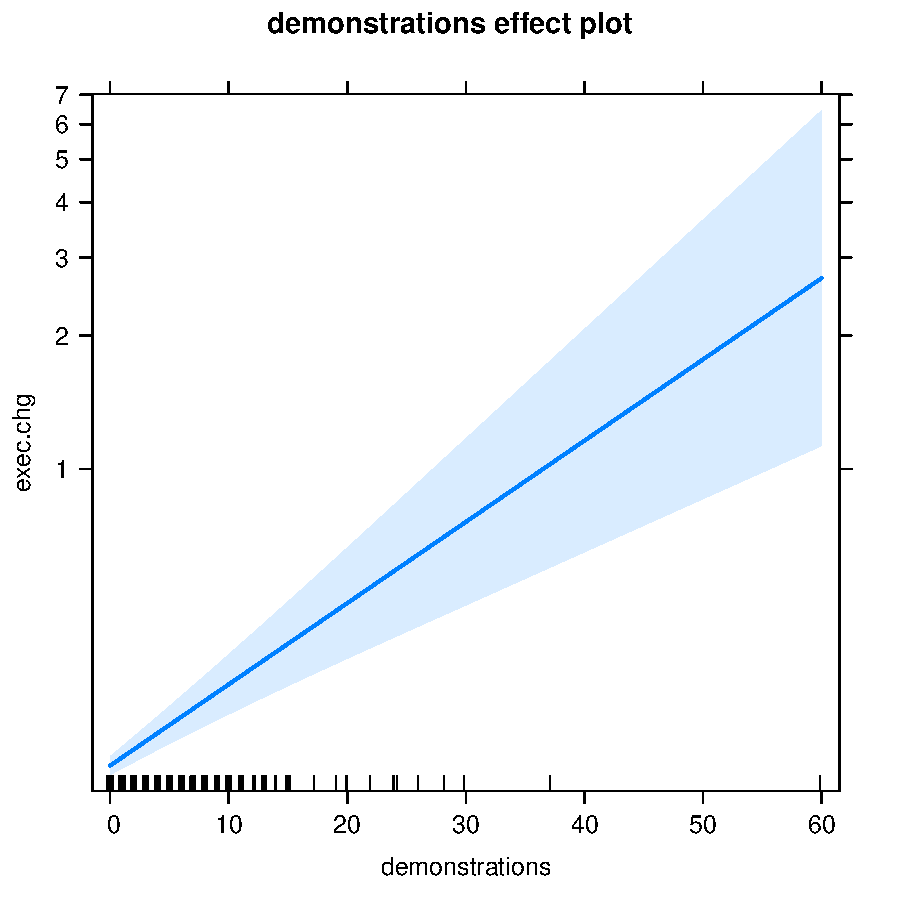
\includegraphics[width=\maxwidth]{figure/pp-1} 

}


\begin{kframe}\begin{alltt}
\hlkwd{plot}\hlstd{(}\hlkwd{effect}\hlstd{(}\hlstr{"guerilla"}\hlstd{, modelo.p))}
\end{alltt}
\end{kframe}

{\centering 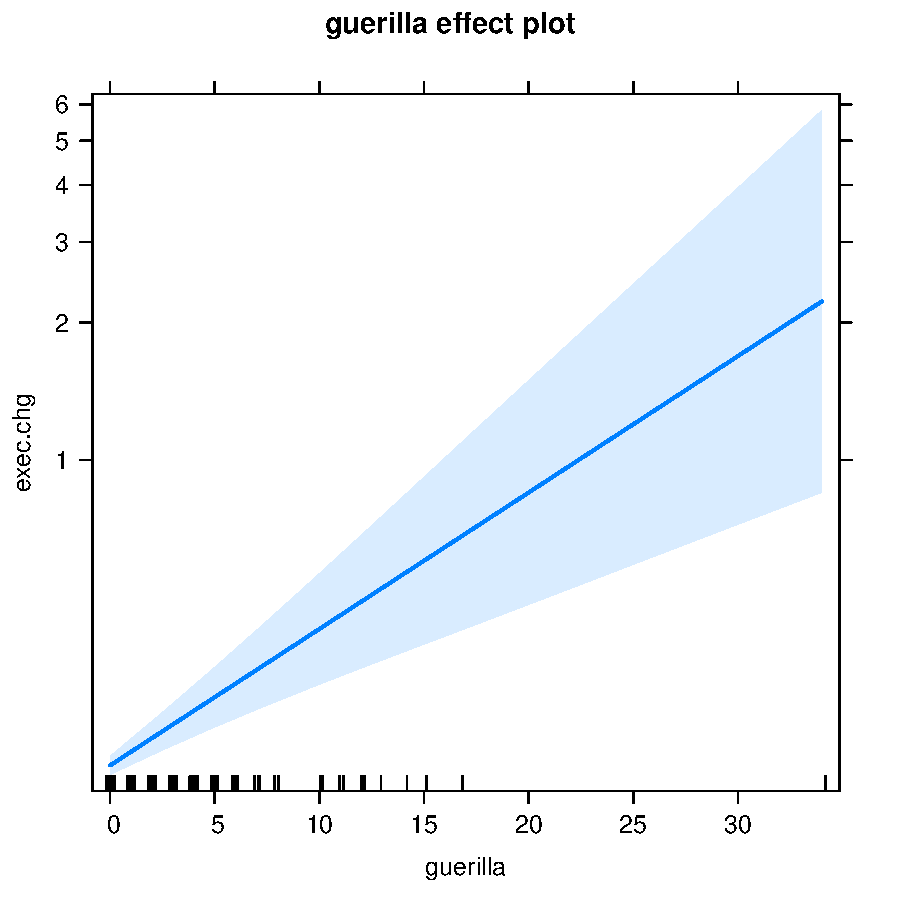
\includegraphics[width=\maxwidth]{figure/pp-2} 

}


\begin{kframe}\begin{alltt}
\hlkwd{plot}\hlstd{(}\hlkwd{effect}\hlstd{(}\hlstr{"regime.type"}\hlstd{, modelo.p))}
\end{alltt}
\end{kframe}

{\centering 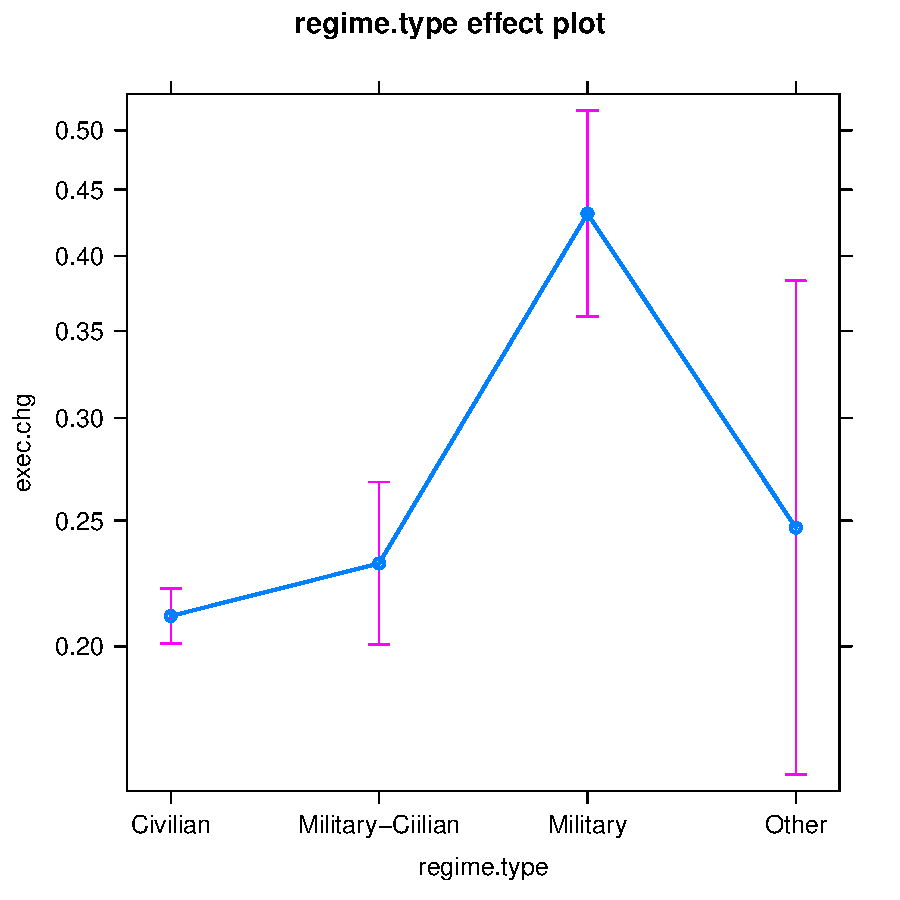
\includegraphics[width=\maxwidth]{figure/pp-3} 

}





Ahora, veamos si tenemos \emph{overdispersion}. Para esto, usaremos el test desarrollado por \textcite{Cameron1990a}. Ellos explican que la hip\'otesis nula $E(y_{i}|\boldsymbol{x}_{i}) = \text{Var}(y_{i}|\boldsymbol{x}_{i})$. Si el p-value es significativo, tendremos evidencia suficiente para sugerir que la media y la varianza no son iguales.


\begin{knitrout}
\definecolor{shadecolor}{rgb}{0.969, 0.969, 0.969}\color{fgcolor}\begin{kframe}
\begin{alltt}
\hlkwd{p_load}\hlstd{(AER)}
\hlkwd{dispersiontest}\hlstd{(modelo.p)}
\end{alltt}
\begin{verbatim}
## 
## 	Overdispersion test
## 
## data:  modelo.p
## z = 5.6944, p-value = 0.000000006192
## alternative hypothesis: true dispersion is greater than 1
## sample estimates:
## dispersion 
##   1.229601
\end{verbatim}
\end{kframe}
\end{knitrout}

El test es altamente significativo, por lo que s\'i tenemos evidencia a favor de overdispersion. Entonces deberemos pasar el modelo Negative-Binomial.


\subsection{Modelo Negative-Binomial}

Muy rara vez el modelo Poisson cumple su supuesto \parencite[230]{Long:1997wv}. Lo que haremos ser\'a generalizar \autoref{poisson:pro}, y permitir que exista heterogenidad no-observada v\'ia la introducci\'on de un residuo $e_{i}$ (que hasta el momento el modelo Poisson no lo permit\'ia).

En consecuencia, ahora tenemos que el ``\emph{rate}'' del modelo Negative-Binomial est\'a dado por,


\begin{equation}\label{nb:mu}
\tilde{\mu}_{i} = \text{exp}(\boldsymbol{x}_{i}\boldsymbol{\beta}) + \text{exp}(\epsilon_{i})
\end{equation}

Nota que ahora $\mu_{i}$ es un vector (i.e. una distribuci\'on), no un escalar. Esto se traduce en el hecho de que tendremos distintos valores de $\mu_{i}$ seg\'un las distintas combinamos de valores en las variables independientes $\boldsymbol{x}_{i}$. 

\paragraph{Supuestos Distribucionales} El supuesto distribucional es que $\text{exp}(\epsilon_{i})$ (o muchas veces llamado el par\'ametro $\delta$)  toma el valor de $E(\text{exp}(\epsilon_{i}))=1$. 

\begin{itemize}
\item De manera muy importante, esta sigue siendo una distribuci\'on Poisson, pero ``modificada'' (de hecho el valor esperado sigue siendo el mismo, s\'olo cambia la varianza). 
\item Nota adem\'as que $\delta$ (como cualquier varianza) es \emph{desconocida} (es un ``\emph{population parameter}''). 
\item Finalmente, parte del supuesto es que $\delta$ se distribuye siguiendo la distribuci\'on Gamma.
\end{itemize}

\paragraph{Contagio} La flexibilidad del modelo Negative-Binomial permite modelar situaciones de {\bf contagio}. Esto se refiere a situaciones donde la probabilidad de obtener ciertas cuentas est\'a correlacionada con el n\'umero de cuentas. Volviendo al ejemplo de \emph{papers} publicados, en la especificaci\'on Negative-Binomial podr\'iamos modelar la situaci\'on donde los acad\'emicos tienen m\'as probabilidades de publicar \emph{papers} mientras m\'as \emph{papers} tengan publicados! Esto se refiere a que el modelo permite tomar en cuenta \emph{data generating processes} que {\bf no asuman independencia estoc\'astica}.

\paragraph{Estimaci\'on}  Ahora procedamos a estimar el modelo.

\begin{knitrout}
\definecolor{shadecolor}{rgb}{0.969, 0.969, 0.969}\color{fgcolor}\begin{kframe}
\begin{alltt}
\hlkwd{p_load}\hlstd{(MASS)}
\hlstd{modelo.nb} \hlkwb{=} \hlkwd{glm.nb}\hlstd{(exec.chg} \hlopt{~} \hlstd{demonstrations} \hlopt{+} \hlstd{guerilla} \hlopt{+} \hlstd{regime.type,} \hlkwc{data}\hlstd{=dat)}
\end{alltt}
\end{kframe}
\end{knitrout}

Y de hecho comparemos ambos modelos,

\begin{kframe}
\begin{alltt}
\hlkwd{p_load}\hlstd{(texreg)}
\hlkwd{texreg}\hlstd{(}\hlkwd{list}\hlstd{(modelo.p, modelo.nb))} \hlcom{# usa "screenreg" no "texreg".}
\end{alltt}
\end{kframe}
\begin{table}
\begin{center}
\begin{tabular}{l c c}
\hline
 & Model 1 & Model 2 \\
\hline
(Intercept)                 & $-1.59^{***}$ & $-1.60^{***}$ \\
                            & $(0.03)$      & $(0.03)$      \\
demonstrations              & $0.04^{***}$  & $0.05^{***}$  \\
                            & $(0.01)$      & $(0.01)$      \\
guerilla                    & $0.07^{***}$  & $0.09^{***}$  \\
                            & $(0.01)$      & $(0.02)$      \\
regime.typeMilitary-Ciilian & $0.09$        & $0.09$        \\
                            & $(0.08)$      & $(0.08)$      \\
regime.typeMilitary         & $0.71^{***}$  & $0.71^{***}$  \\
                            & $(0.10)$      & $(0.11)$      \\
regime.typeOther            & $0.16$        & $0.15$        \\
                            & $(0.23)$      & $(0.25)$      \\
\hline
AIC                         & $10073.24$    & $9954.78$     \\
BIC                         & $10115.64$    & $10004.25$    \\
Log Likelihood              & $-5030.62$    & $-4970.39$    \\
Deviance                    & $6695.27$     & $5398.93$     \\
Num. obs.                   & $8659$        & $8659$        \\
\hline
\multicolumn{3}{l}{\scriptsize{$^{***}p<0.001$; $^{**}p<0.01$; $^{*}p<0.05$}}
\end{tabular}
\caption{Statistical models}
\label{table:coefficients}
\end{center}
\end{table}


Encontramos---sin sorpresa---que los modelos son altamente parecidos. 

\paragraph{Interpretaci\'on} En cualquier caso, ya sabemos que la tabla poco valor tiene. Ahora procederemos a estimar los \emph{predicted probabilities}.


\begin{kframe}
\begin{alltt}
\hlkwd{p_load}\hlstd{(effects)}
\hlkwd{plot}\hlstd{(}\hlkwd{effect}\hlstd{(}\hlstr{"demonstrations"}\hlstd{, modelo.nb))}
\end{alltt}
\end{kframe}

{\centering 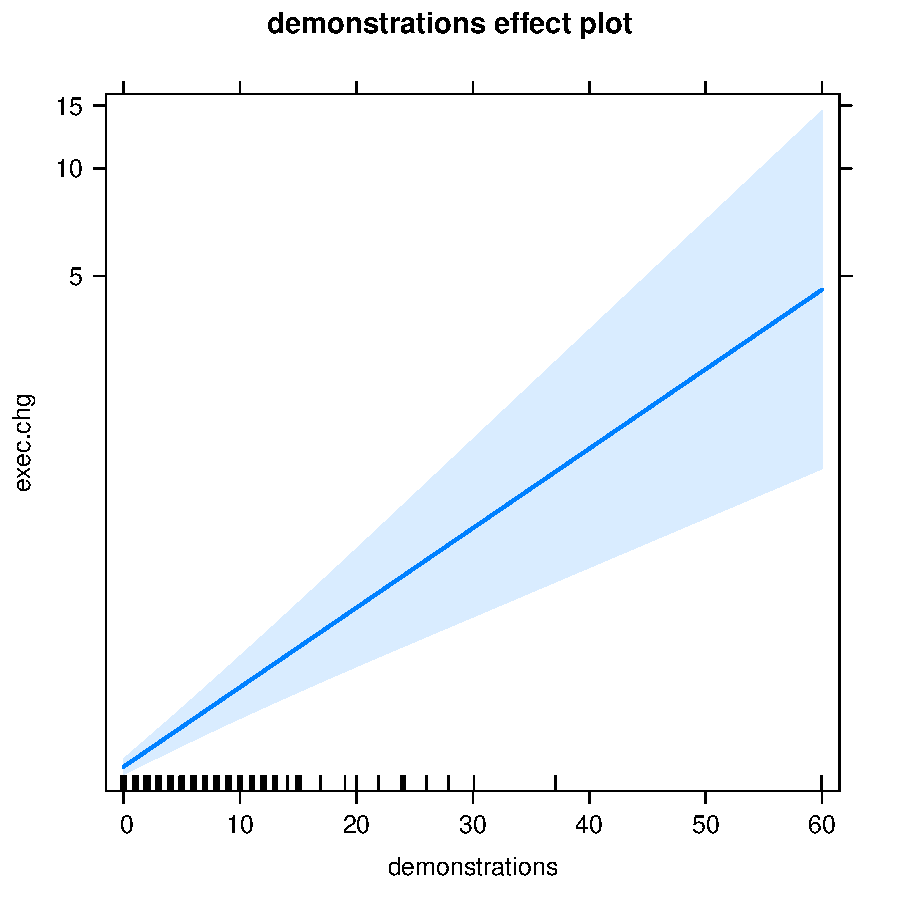
\includegraphics[width=\maxwidth]{figure/pp2-1} 

}


\begin{kframe}\begin{alltt}
\hlkwd{plot}\hlstd{(}\hlkwd{effect}\hlstd{(}\hlstr{"guerilla"}\hlstd{, modelo.nb))}
\end{alltt}
\end{kframe}

{\centering 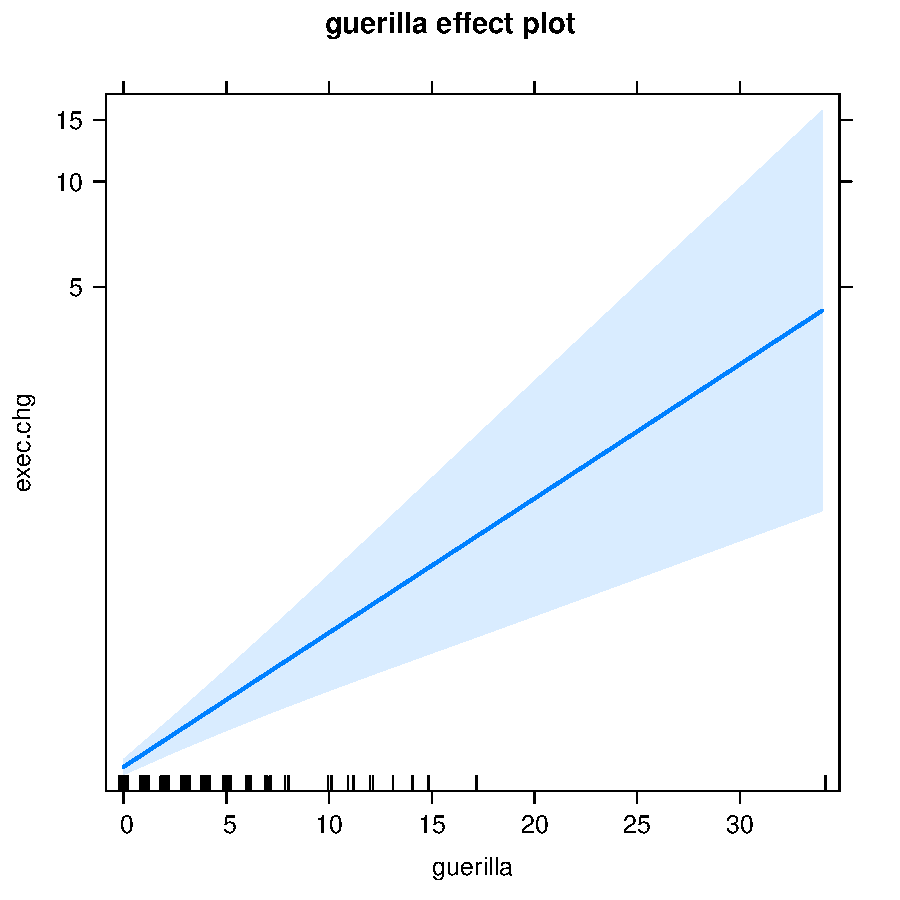
\includegraphics[width=\maxwidth]{figure/pp2-2} 

}


\begin{kframe}\begin{alltt}
\hlkwd{plot}\hlstd{(}\hlkwd{effect}\hlstd{(}\hlstr{"regime.type"}\hlstd{, modelo.nb))}
\end{alltt}
\end{kframe}

{\centering 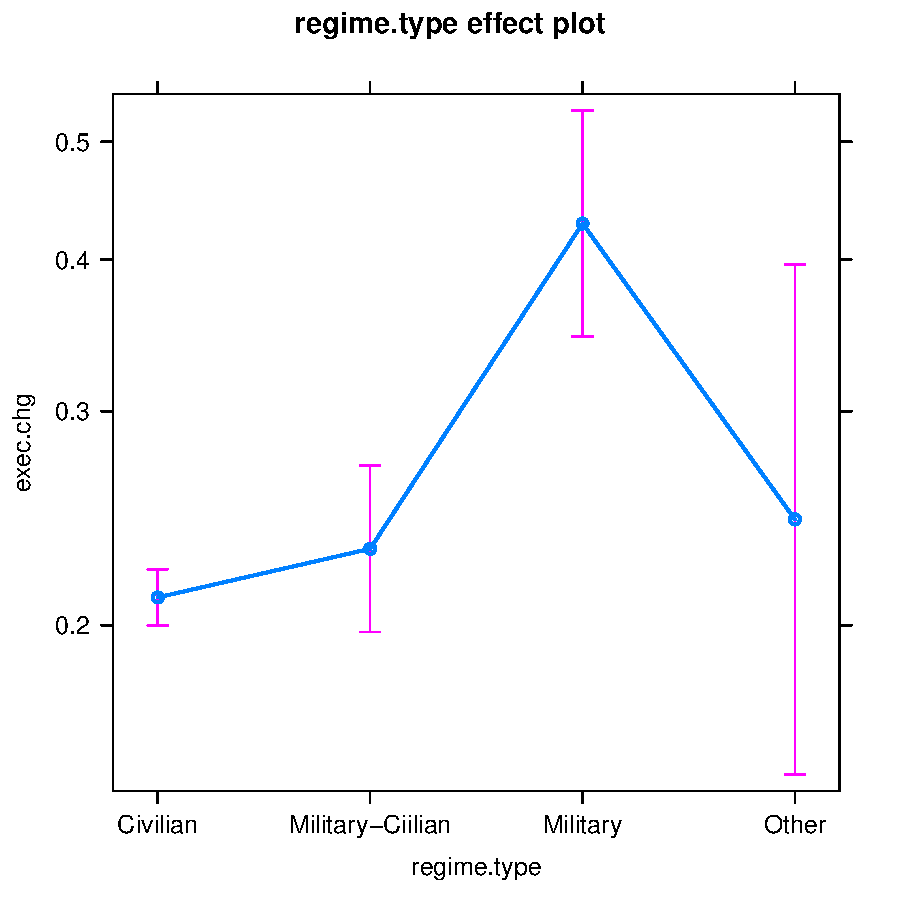
\includegraphics[width=\maxwidth]{figure/pp2-3} 

}






\begin{knitrout}
\definecolor{shadecolor}{rgb}{0.969, 0.969, 0.969}\color{fgcolor}\begin{kframe}
\begin{alltt}
\hlstd{knitr}\hlopt{::}\hlkwd{purl}\hlstd{(}\hlstr{'Multinomial.Rnw'}\hlstd{)}
\end{alltt}


{\ttfamily\noindent\bfseries\color{errorcolor}{\#\# Error in file(con, "{}r"{}): no se puede abrir la conexi'on}}\begin{alltt}
\hlkwd{Stangle}\hlstd{(}\hlstr{'Multinomial.Rnw'}\hlstd{)}
\end{alltt}


{\ttfamily\noindent\bfseries\color{errorcolor}{\#\# Error in SweaveReadFile(file, syntax, encoding = encoding): no Sweave file with name 'Multinomial.Rnw' found}}\end{kframe}
\end{knitrout}

%\newpage
%\paragraph{}
%\paragraph{}
%\pagenumbering{Roman}
%\setcounter{page}{1}
%\printbibliography



\end{document}

